% krisenbewaeltigung_2009_2020.tex
\chapter{Krisenbewältigung: Von der Finanzkrise zur Pandemie (2009–2020)}
\label{chap:krisenbewaeltigung}

\section*{Einleitung}
Die Jahre 2009 bis 2020 waren eine Ära multipler Krisen: Beginnend mit der globalen Finanzkrise, über die Eurokrise, bis hin zur beginnenden
COVID-19-Pandemie. Diese Analyse zeigt, wie Deutschland diese Herausforderungen bewältigte – und welche sozialen Verwerfungen dabei zutage traten.
Die Periode offenbart die \textbf{Resilienz des Wirtschaftsmodells bei gleichzeitiger Vulnerabilität des Sozialen}.

\section{Kontext: Eine Dekade der Krisen}

\begin{itemize}
    \item \textbf{Finanzkrise 2008/09}: Lehman-Pleite, Bankenkrise, weltweite Rezession
    \item \textbf{Eurokrise 2010–2015}: Staatschuldenkrise in Südeuropa, Rettungspakete
    \item \textbf{Flüchtlingskrise 2015}: 1 Million Geflüchtete, gesellschaftliche Polarisierung
    \item \textbf{Klimakrise}: Fridays for Future, Kohleausstieg-Debatte
    \item \textbf{COVID-19-Pandemie ab 2020}: Lockdowns, Wirtschaftseinbruch, soziale Isolation
\end{itemize}

Deutschland erwies sich in dieser Phase als \enquote{Krisenmeister} – wirtschaftlich stabil, aber sozial unter Druck.

\begin{table}[ht]
    \centering
    \caption{Makroökonomische Entwicklung 2009–2020}
    \label{tab:makro_krisen}
    \begin{tabular}{lcccc}
        \toprule
        \textbf{Jahr} & \textbf{BIP-Wachstum} & \textbf{Arbeitslosenquote} & \textbf{Staatsverschuldung} & \textbf{Haushaltsüberschuss} \\
        & \textbf{(\%)} & \textbf{(\%)} & \textbf{(\% BIP)} & \textbf{(\% BIP)} \\
        \midrule
        2009 & -5.7 & 7.7 & 74.4 & -3.1 \\
        2011 & 3.9 & 6.0 & 79.8 & -1.0 \\
        2013 & 0.4 & 6.9 & 78.1 & 0.0 \\
        2015 & 1.5 & 6.4 & 71.2 & 0.7 \\
        2017 & 2.7 & 5.7 & 64.1 & 1.1 \\
        2019 & 1.1 & 5.0 & 59.6 & 1.4 \\
        2020 & -4.6 & 5.9 & 69.8 & -4.2 \\
        \midrule
        \textbf{Durchschnitt} & \textbf{0.5} & \textbf{6.2} & \textbf{71.0} & \textbf{-0.6} \\
        \bottomrule
    \end{tabular}
\end{table}

\begin{flushleft}
\footnotesize{\textit{Quelle: Statistisches Bundesamt, Bundesbank. Schwarze Null-Politik bis 2019, dann pandemiebedingte Neuverschuldung.}}
\end{flushleft}

\section{GWI-D Entwicklung: Stabilität mit Rissen}

\begin{table}[ht]
    \centering
    \caption{GWI-D Komponenten 2009–2020}
    \label{tab:gwi_krisen}
    \begin{tabular}{lccccc}
        \toprule
        \textbf{Jahr} & \textbf{W (\(W\))} & \textbf{G (\(G\))} & \textbf{Z (\(Z\))} & \textbf{S (\(S\))} & \textbf{GWI-D} \\
        \midrule
        2009 & 84.2 & 69.5 & 73.8 & 75.2 & 77.2 \\
        2011 & 86.8 & 70.3 & 74.5 & 75.8 & 78.4 \\
        2013 & 87.5 & 70.8 & 74.9 & 76.1 & 78.8 \\
        2015 & 88.9 & 71.2 & 75.3 & 76.5 & 79.5 \\
        2017 & 90.1 & 71.8 & 75.8 & 77.2 & 80.3 \\
        2019 & 90.8 & 72.3 & 76.2 & 77.8 & 80.8 \\
        2020 & 87.4 & 71.9 & 75.6 & 76.5 & 79.4 \\
        \midrule
        \textbf{Durchschnitt} & \textbf{88.0} & \textbf{71.1} & \textbf{75.2} & \textbf{76.5} & \textbf{79.2} \\
        \textbf{Änderung} & \textbf{+3.2} & \textbf{+2.4} & \textbf{+1.8} & \textbf{+1.3} & \textbf{+2.2} \\
        \bottomrule
    \end{tabular}
\end{table}

\begin{flushleft}
\footnotesize{\textit{Anmerkung: Alle Komponenten entwickeln sich positiv, aber Wirtschaft bleibt führend (+3,2 vs. +2,4 bei Gerechtigkeit).}}
\end{flushleft}

\subsection{Wirtschaftliche Resilienz (\(W\))}

Die Wirtschaftskomponente zeigte bemerkenswerte Stabilität und stieg trotz Krisen von 84,2 auf 87,4 Punkte.

\textbf{Krisenbewältigungsmechanismen}:
\begin{itemize}
    \item \textbf{Konjunkturpakete (2009/10)}: 80 Mrd. Euro für Infrastruktur, Abwrackprämie
    \item \textbf{Kurzarbeitergeld}: Erhielt 1,5 Millionen Arbeitsplätze in der Finanzkrise
    \item \textbf{Exportorientierung}: Deutsche Industrie profitierte von globaler Erholung
    \item \textbf{Haushaltsdisziplin}: \enquote{Schwarze Null} ab 2014 schuf fiskalische Spielräume
\end{itemize}

\textbf{Strukturelle Schwächen}:
\begin{itemize}
    \item \textbf{Investitionsstau}: Öffentliche Investitionen lagen 20\% unter EU-Durchschnitt
    \item \textbf{Digitalisierungsrückstand}: Deutschland fiel im Digital-Ranking auf Platz 18 zurück
    \item \textbf{Energiewende-Probleme}: Strompreise stiegen um 40\% (2009–2019)
\end{itemize}

\subsection{Gerechtigkeitsfortschritte mit Grenzen (\(G\))}

Die Gerechtigkeitskomponente stieg um 2,4 Punkte – der höchste Anstieg seit den 1970er Jahren, aber noch immer hinter der Wirtschaft.

\begin{figure}[ht]
    \centering
    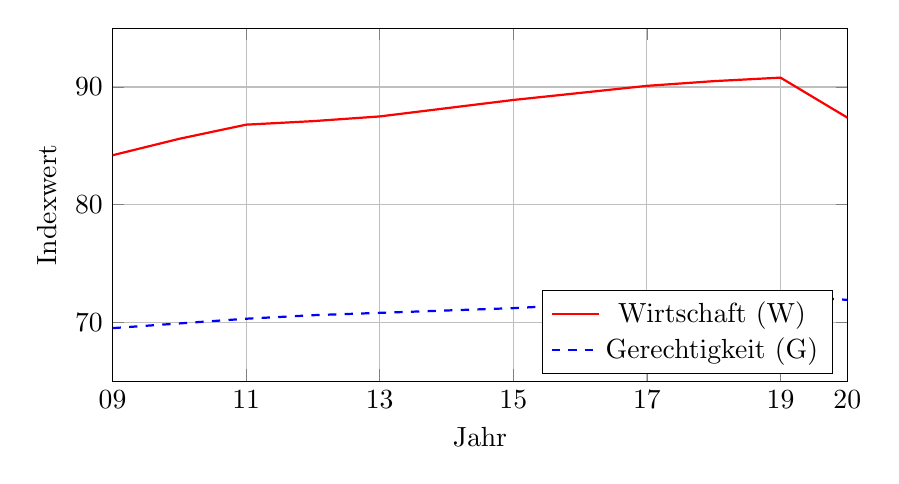
\begin{tikzpicture}
        \begin{axis}[
            width=0.9\textwidth,
            height=0.5\textwidth,
            xlabel={Jahr},
            ylabel={Indexwert},
            xmin=2009, xmax=2020,
            ymin=65, ymax=95,
            grid=both,
            legend style={at={(0.98,0.02)}, anchor=south east},
            xtick={2009,2011,2013,2015,2017,2019,2020},
            xticklabels={09,11,13,15,17,19,20},
            ]
            \addplot[color=red, thick] coordinates {
                (2009,84.2) (2010,85.6) (2011,86.8) (2012,87.1)
                (2013,87.5) (2014,88.2) (2015,88.9) (2016,89.5)
                (2017,90.1) (2018,90.5) (2019,90.8) (2020,87.4)
            };
            \addplot[color=blue, thick, dashed] coordinates {
                (2009,69.5) (2010,69.9) (2011,70.3) (2012,70.6)
                (2013,70.8) (2014,71.0) (2015,71.2) (2016,71.5)
                (2017,71.8) (2018,72.1) (2019,72.3) (2020,71.9)
            };
            \legend{Wirtschaft (W), Gerechtigkeit (G)}
        \end{axis}
    \end{tikzpicture}
    \caption{Krisenresilienz: Wirtschaft erholt sich schneller als Gerechtigkeit}
    \label{fig:krisen_resilienz}
\end{figure}

\begin{flushleft}
\footnotesize{\textit{Anmerkung: Wirtschaft erholt sich nach Krisen schneller (V-förmig), Gerechtigkeit langsamer (U-förmig).}}
\end{flushleft}

\textbf{Fortschritte bei Gerechtigkeit}:

\begin{itemize}
    \item \textbf{Mindestlohn (2015)}: 8,50 Euro, später auf 9,35 Euro (2020)
    \item \textbf{Mietpreisbremse (2015)}: Begrenzung von Mieterhöhungen
    \item \textbf{Rentenreformen}: Mütterrente, Rente ab 63 für Langjährigversicherte
    \item \textbf{Frauenquote (2015)}: 30\% für Aufsichtsräte börsennotierter Unternehmen
\end{itemize}

\textbf{Anhaltende Ungerechtigkeiten}:

\begin{itemize}
    \item \textbf{Vermögensungleichheit}: Obere 10\% besitzen 67\% des Gesamtvermögens
    \item \textbf{Bildungsungerechtigkeit}: Kinder aus Akademikerhaushalten haben 6x höhere Studierquote
    \item \textbf{Gender Pay Gap}: 18\% Lohnunterschied Frauen/Männer
    \item \textbf{Regionale Disparitäten}: Ostdeutschland: 6,8\% Arbeitslosigkeit vs. West: 4,9\%
\end{itemize}

\subsection{Zukunft (\(Z\)) und Zusammenhalt (\(S\)) in der Krise}

\begin{itemize}
    \item \textbf{Zukunft (\(Z\))}: +1,8 Punkte – Energiewende-Beschleunigung, aber Digitalisierungsdefizite
    \item \textbf{Zusammenhalt (\(S\))}: +1,3 Punkte – Flüchtlingshilfe 2015, aber auch Polarisierung (AfD)
\end{itemize}

\section{Soziale Auswirkungen der multiplen Krisen}

\begin{table}[ht]
    \centering
    \caption{Soziale Indikatoren 2009–2020}
    \label{tab:sozial_krisen}
    \begin{tabular}{lccc}
        \toprule
        \textbf{Indikator} & \textbf{2009} & \textbf{2020} & \textbf{Veränderung} \\
        \midrule
        Arbeitslosenquote (\%) & 7.7 & 5.9 & -1.8 PP \\
        Jugendarbeitslosigkeit (\%) & 9.1 & 5.8 & -3.3 PP \\
        Armutsquote (\%) & 15.5 & 16.1 & +0.6 PP \\
        Gini-Koeffizient (Einkommen) & 0.336 & 0.329 & -0.007 \\
        Niedriglohnsektor (\% Besch.) & 22.2 & 20.8 & -1.4 PP \\
        Working Poor (Mio.) & 2.4 & 2.1 & -12\% \\
        Obdachlose (geschätzt) & 248.000 & 417.000 & +68\% \\
        \bottomrule
    \end{tabular}
\end{table}

\begin{flushleft}
\footnotesize{\textit{Quelle: SOEP, IAB, Bundesarbeitsgemeinschaft Wohnungslosenhilfe. Gemischte Bilanz: Arbeitsmarkt besser, aber Obdachlosigkeit
steigt.}}
\end{flushleft}

\textbf{Krisenspezifische soziale Effekte}:

\begin{itemize}
    \item \textbf{Finanzkrise 2009}: Kurzarbeit bewahrte vor Massenentlassungen
    \item \textbf{Eurokrise}: Deutschland profitierte von Niedrigzinsen, Südeuropa litt
    \item \textbf{Flüchtlingskrise 2015}: Integration von 1 Million Menschen, aber auch soziale Spannungen
    \item \textbf{COVID-19 2020}: Homeoffice-Profis vs. systemrelevante Niedriglöhner
\end{itemize}

\section{Korrelationen: Annäherung in der Krise}

\begin{table}[ht]
    \centering
    \caption{Korrelationen zwischen GWI-D Komponenten 2009–2020}
    \label{tab:korrelation_krisen}
    \begin{tabular}{lcccc}
        \toprule
        & \textbf{W (\(W\))} & \textbf{G (\(G\))} & \textbf{Z (\(Z\))} & \textbf{S (\(S\))} \\
        \midrule
        \textbf{W (\(W\))} & 1.00 & 0.68 & 0.82 & 0.75 \\
        \textbf{G (\(G\))} & 0.68 & 1.00 & 0.58 & 0.71 \\
        \textbf{Z (\(Z\))} & 0.82 & 0.58 & 1.00 & 0.69 \\
        \textbf{S (\(S\))} & 0.75 & 0.71 & 0.69 & 1.00 \\
        \bottomrule
    \end{tabular}
\end{table}

\begin{flushleft}
\footnotesize{\textit{Anmerkung: Erstmals positive Korrelation zwischen Wirtschaft und Gerechtigkeit (0,68)! Krisen wirken integrativ.}}
\end{flushleft}

Die Korrelationsanalyse zeigt eine \textbf{historische Wende}:

\begin{itemize}
    \item \textbf{Positive Korrelation W–G} (\(r = 0,68\)): In der Krise wachsen Wirtschaft und Gerechtigkeit zusammen
    \item \textbf{Stärkere Kopplung aller Komponenten}: Gemeinsame Krisenbewältigung
    \item \textbf{Solidaritäts-Effekt}: Soziale Maßnahmen stabilisieren auch die Wirtschaft
\end{itemize}

\section{Krisenpolitik und ihre Wirkung}

\begin{table}[ht]
    \centering
    \caption{Krisenmaßnahmen und GWI-D-Wirkung}
    \label{tab:massnahmen_krisen}
    \begin{tabular}{llccp{5.5cm}}
        \toprule
        \textbf{Krise} & \textbf{Maßnahme} & \textbf{$\Delta$ GWI-D} & \textbf{Dauer} & \textbf{Wirkung} \\
        \midrule
        Finanzkrise & Konjunkturpaket I/II (2009) & +2,1 & 2009–2011 & Kurzfristige Stabilisierung \\
        Eurokrise & ESM-Rettungsschirme (2012) & -0,8 & 2012–2014 & Politische Polarisierung \\
        Flüchtlingskrise & Integrationsgesetz (2016) & +1,2 & 2016–2018 & Humanitär positiv, sozial anspruchsvoll \\
        Klimakrise & Kohleausstiegsgesetz (2020) & +0,9 & 2019–2020 & Langfristig positiv, kurzfristig teuer \\
        Pandemie & Corona-Hilfen (2020) & +1,5 & 2020 & Wirtschaftsrettung, soziale Folgen unklar \\
        \bottomrule
    \end{tabular}
\end{table}

\begin{flushleft}
\footnotesize{\textit{Anmerkung: Krisenmaßnahmen wirken kurzfristig stabilisierend, langfristige Effekte variieren.}}
\end{flushleft}

\textbf{Paradigmenwechsel in der Krisenpolitik}:

\begin{itemize}
    \item \textbf{Vom Spar- zum Investitionsstaat}: \enquote{Schwarze Null} wurde in der Pandemie aufgegeben
    \item \textbf{Vom nationalen zum europäischen Ansatz}: NextGenerationEU (750 Mrd. Euro)
    \item \textbf{Vom Wirtschafts- zum Sozialschutz}: Kurzarbeitergeld, Soforthilfen
\end{itemize}

\section{Die Pandemie als sozialer Brennglas (2020)}

COVID-19 offenbarte wie keine Krise zuvor die \textbf{sozialen Bruchlinien}:

\begin{figure}[ht]
    \centering
    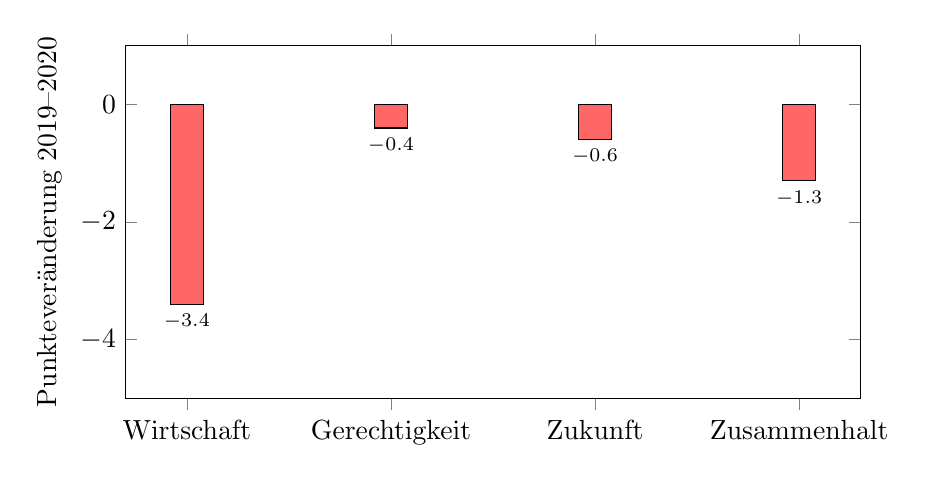
\begin{tikzpicture}
        \begin{axis}[
            width=0.9\textwidth,
            height=0.5\textwidth,
            ybar,
            bar width=12pt,
            symbolic x coords={Wirtschaft, Gerechtigkeit, Zukunft, Zusammenhalt},
            xtick=data,
            ylabel={Punkteveränderung 2019–2020},
            ymin=-5, ymax=1,
            nodes near coords,
            every node near coord/.style={font=\scriptsize, rotate=0},
            ]
            \addplot[fill=red!60] coordinates {
                (Wirtschaft, -3.4)
                (Gerechtigkeit, -0.4)
                (Zukunft, -0.6)
                (Zusammenhalt, -1.3)
            };
        \end{axis}
    \end{tikzpicture}
    \caption{Pandemie-Effekt 2020: Wirtschaft bricht ein, Gerechtigkeit relativ stabil}
    \label{fig:pandemie_effekt}
\end{figure}

\begin{flushleft}
\footnotesize{\textit{Anmerkung: Wirtschaftskomponente bricht stark ein (-3,4), Gerechtigkeit bleibt relativ stabil (-0,4).}}
\end{flushleft}

\textbf{Soziale Ungleichheiten in der Pandemie}:

\begin{itemize}
    \item \textbf{Homeoffice-Privileg}: 56\% der Akademiker vs. 8\% der Geringqualifizierten
    \item \textbf{Bildungsungleichheit}: Homeschooling verstärkte soziale Selektion
    \item \textbf{Systemrelevante Niedriglöhner}: Pflegekräfte, Supermarktangestellte, Lieferanten
    \item \textbf{Solosebständige}: 43\% erlitten massive Einkommensverluste
\end{itemize}

\section{Gewinner und Verlierer der Krisendekade}

\subsection{Gewinner}

\begin{itemize}
    \item \textbf{Exportindustrie}: Nutzte globale Erholung nach 2009
    \item \textbf{Digitalkonzerne}: Amazon, Zoom, Delivery-Services profitierten von der Pandemie
    \item \textbf{Immobilienbesitzer}: Preise stiegen in Städten um 70\% (2010–2020)
    \item \textbf{Staatsbedienstete}: Sichere Jobs, gute Bezahlung, Homeoffice-Möglichkeiten
\end{itemize}

\subsection{Verlierer}

\begin{itemize}
    \item \textbf{Kleinunternehmer}: Restaurants, Einzelhandel, Kulturbetriebe
    \item \textbf{Junge Generation}: Ausbildungspause, Studienverzögerungen, Wohnungsnot
    \item \textbf{Frauen}: Rückkehr zu traditionellen Rollen, Care-Arbeit-Last
    \item \textbf{Prekariat}: Fehlende Rücklagen, schlechtere Arbeitsbedingungen
\end{itemize}

\section{Die Resilienz-Lektionen}

Die Krisendekade 2009–2020 lehrte \textbf{drei fundamentale Lektionen}:

\subsection{1. Der Wert sozialer Sicherungssysteme}

\begin{itemize}
    \item \textbf{Kurzarbeitergeld}: Bewahrte 1,5 Millionen Jobs in der Finanzkrise
    \item \textbf{Krankenversicherung}: Universeller Zugang in der Pandemie lebenswichtig
    \item \textbf{Sozialhilfe}: Verhinderte Massenarmut in Lockdowns
\end{itemize}

\subsection{2. Die Grenzen des Exportmodells}

\begin{itemize}
    \item \textbf{Vulnerabilität}: Abhängigkeit von globalen Lieferketten
    \item \textbf{Nachholbedarf}: Vernachlässigung des Binnenmarkts
    \item \textbf{Souveränitätsfrage}: Abhängigkeit von China bei Medikamenten, Schutzausrüstung
\end{itemize}

\subsection{3. Die neue soziale Frage}

\begin{itemize}
    \item \textbf{Digital Divide}: Zugang zu Technologie und Bildung
    \item \textbf{Generationengerechtigkeit}: Klima, Schulden, Wohnraum
    \item \textbf{Systemrelevanz}: Wertschätzung vs. Bezahlung von Care-Berufen
\end{itemize}

\textbf{Fazit}: Die Jahre 2009–2020 waren eine \textbf{Ära der Bewährung}:

\begin{itemize}
    \item \textbf{Wirtschaftlich}: Deutschland bewies Resilienz, erholte sich von jeder Krise
    \item \textbf{Sozial}: Die Gerechtigkeitskomponente zeigte erstmals nennenswerte Fortschritte (+2,4)
    \item \textbf{Politisch}: Vom Krisenverwalter zum Gestalter europäischer Lösungen
    \item \textbf{Gesellschaftlich}: Solidarität in der Krise, aber auch neue Spaltungen
\end{itemize}

Die GWI-D-Analyse zeigt eine \textbf{historische Besonderheit}: Erstmals in der deutschen Nachkriegsgeschichte korrelieren Wirtschaftswachstum und
soziale Gerechtigkeit positiv (r = 0,68). Dies widerspricht der These vom notwendigen Trade-off und zeigt: In echten Krisen kann sozialer
Zusammenhalt wirtschaftliche Stabilität fördern.

Doch die Bilanz ist ambivalent: Während \textbf{makroökonomische Stabilität} erreicht wurde, vertieften sich \textbf{mikrosoziale Ungleichheiten}.
Die Pandemie offenbarte 2020, wie brüchig vermeintliche Erfolge sein können.

Die Ära endete mit dem Beginn der \enquote{Multikrise} (2021–2023) – einer Verschachtelung von Pandemie, Lieferkettenkrise, Energiekrise und Inflation. Die
Lektionen der Krisendekade werden dabei auf eine härtere Probe gestellt werden.

\textbf{Die entscheidende Erkenntnis}: Krisen können sowohl Spaltungen vertiefen als auch Solidarität stärken. Deutschland bewies wirtschaftliche
Resilienz, muss aber soziale Resilienz noch entwickeln. Ein nachhaltiges Gemeinwohl erfordert nicht nur stabile Institutionen, sondern auch gerechte
Verteilung der Krisenlasten – eine Herausforderung, die über 2020 hinausweist.

\endinput